\documentclass[a4paper,landscape]{article} % Página más ancha
\usepackage{tikz}
\usepackage[margin=1.5cm]{geometry} % Márgenes reducidos para más espacio

\begin{document}

\begin{center}
    \textbf{Distancia Euclidiana vs Distancia Manhattan}
\end{center}

\begin{center}
    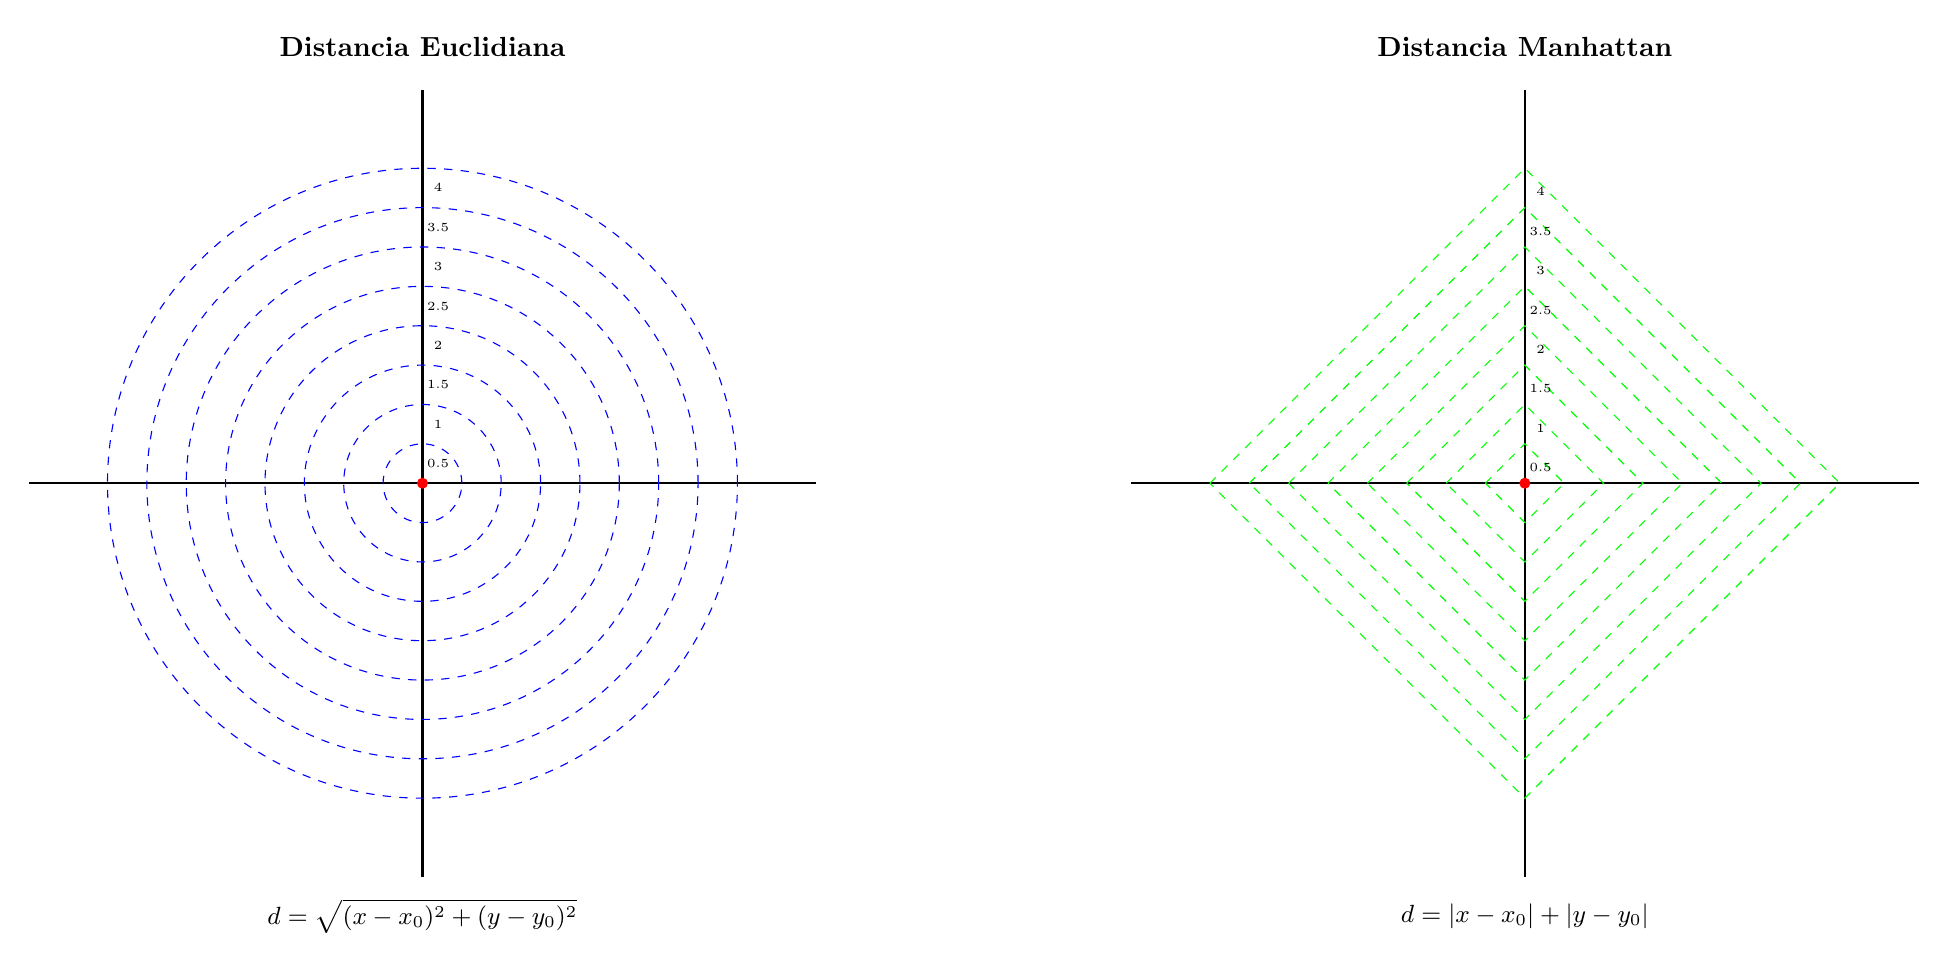
\begin{tikzpicture}[scale=1] % Ajuste de escala general

        % Subgráfico: Distancia Euclidiana
        \begin{scope}[shift={(-7,0)}] % Más separación entre gráficos
            \draw[thick] (-5,0) -- (5,0); % Eje X
            \draw[thick] (0,-5) -- (0,5); % Eje Y
            \foreach \r in {0.5,1,1.5,2,2.5,3,3.5,4} {
                \draw[blue, dashed] (0,0) circle (\r);
                \node[black, scale=0.9] at (0.2,\r-0.25) {\tiny \r}; % Números más pequeños y más a la derecha
            }
            \fill[red] (0,0) circle (2pt);
            \node at (0,-5.5) {\small $d = \sqrt{(x - x_0)^2 + (y - y_0)^2}$};
            \node[above] at (0,5.3) {\textbf{Distancia Euclidiana}};
        \end{scope}

        % Subgráfico: Distancia Manhattan
        \begin{scope}[shift={(7,0)}] % Más separación entre gráficos
            \draw[thick] (-5,0) -- (5,0); % Eje X
            \draw[thick] (0,-5) -- (0,5); % Eje Y
            \foreach \r in {0.5,1,1.5,2,2.5,3,3.5,4} {
                \draw[green, dashed] (-\r,0) -- (0,\r) -- (\r,0) -- (0,-\r) -- cycle;
                \node[black, scale=0.9] at (0.2,\r-0.3) {\tiny \r}; % Números más pequeños y mejor posicionados
            }
            \fill[red] (0,0) circle (2pt);
            \node at (0,-5.5) {\small $d = |x - x_0| + |y - y_0|$};
            \node[above] at (0,5.3) {\textbf{Distancia Manhattan}};
        \end{scope}

    \end{tikzpicture}
\end{center}

\end{document}
